\documentclass[12pt]{report}

\usepackage{import}
\import{../}{preamble.tex}

\begin{document}
\begin{flushleft}
    
\section*{What is Macroeconomics?}
Macroeconomics is the study of \textit{aggregate economic fluctuations}. Key
points of study are features like output, details of the labour market like 
unemployment and inflation. \par
Through studying it, we can examine how governments should respond to 
recessions why countries are rich or poor and how policy can interact with 
economic structures. \par
A major event leading to the development of macroeconomics as a field was the
greate depression, which lead John Maynard Keynes to develop Keynesian theory,
a fundamental part of macroeconomics, and covered in some detail in this 
course.

\bigskip
Major topics of this subject include
\begin{itemize}
    \item Measurement and evaluation of economies
    \item Short or long run economic cycles
    \item Long term growth and development
    \item Effects and behaviour of the global economy
\end{itemize}

\section*{Measurement}
Understanding the state of an economy relies upon accurate measurement of it,
and this understanding is essential to effectively regulating and improving an
economy. Theories with respect to measurement of economies are developed 
according to the study of data.

\subsection*{GDP}
GDP or Gross Domestic Product is a measure of the output of an economy over 
time. The precise definition used in this course is that GDP is the 
\textit{market value} of the \textit{final goods} produced in a country 
during a given time period. GDP is a useful measure of market activity, which
can be used to document change in an economy, compare between economies, and
evaluate the performance of an economy with respect to assorted variables. GDP
is a kind of summary of the performance of an economy. \par
Richard Stone, one of the core forces behind the development of the concept of
GDP was awarded the 1984 Nobel Prize in economics for his efforts.

\subsubsection*{Market Value}
Market value is a way to describe the output of an economy across a wide range
of different goods. The most common form of market value is the financial value
of goods. While this measure is generally quite good, it ignores household 
production as well as grey or black market activities. \par
Because government production has no market price, it is usually valued at
cost of production. This covers public goods such as education, defence and 
public health services.

\subsubsection*{Final Goods and Services}
GDP calculations consider only end products, ignoring constituent goods. For 
example while the loaf of bread sold by a bakery is counted, the flour 
purchased by the bakery and the wheat used to produce that flower is not. This
is done to avoid double counting the contributions of earlier stages. \par
In addition, resold goods are ignored. Second-hand houses or cars are ignored.
Financial assets, such as shares are not a good or service, so they are also
ignored.

\bigskip
GDP considers production in a region; goods produced by international 
businesses in Australia are counted toward Australian GDP while goods produced
internationally by Australian businesses are not.

\subsubsection*{Measurement of GDP}
There are three methods of calculating GDP. These are
\begin{itemize}
    \item Income
    \item Expenditure
    \item Production
\end{itemize}
They should theoretically be equivalent, but practically vary by small margins
due to differences in collection methodology and other real world 
inconveniences.

\subsubsection*{Income}
Every time a good is purchased, money is transferred from a consumer to a
producer. This money is transferred to the firm, which distributes it between
the workers at the firm and the owners of the firm.
\[Y = wL + rK\]
Here, \(Y\) is the GDP, \(w\) is the labour income, \(L\) is the hours worked,
\(r\) is the rental rate and \(K\) is the total capital. Rental rate describes
the amount a production owner earns per unit capital invested into a business.
\par
This method allows examination of the division between capital owners and 
labour providers (workers). Through this examination, one can observe that over
time the share of wealth earned by workers has declined.

\subsubsection*{Expenditure}
The expenditure method examines the amount spent by each group from among four
sectors in the local economy. Each of these is a subtly different form of 
spending.
\begin{itemize}
    \item Houshold sector, which accounts for everyday purchases.
    \item Business sector, which covers investment by businesses.
    \item Government sector, which includes government expenditure less transer
        payments like pension or unemployment benefits.
    \item Overseas sector, which totals net exports (exports less imports).
\end{itemize}
The equation for this sum is
\[Y = C + I + G + X - M\]
Where once again \(Y\) denotes GDP, \(X\) denotes exports, \(M\) is imports and
the other symbols are the remaining three sectors. \par
This measure has the benefit of allowing the examination of consumption versus
investment for instance.

\subsubsection*{Production}
The production method uses a \textit{value added approach}, examining the 
amount of value each producer in an economy. For example, considering a \$3 
loaf of bread.
\begin{itemize}
    \item The bread may have been produced from \$2 worth of flour. Therefore
        the baker add \$1 in value.
    \item The flour may have been milled from \$1 worth of wheat. Therefore the
        miller added \$1 in value.
    \item The farmer, in producing the wheat created \$1 worth of value.
    \item Thus, the total value added throughout production of the loaf of 
        bread was \$3.
\end{itemize}
This approach allows easy comparison between different industries in an 
economy, by considering how much value was added by each industry.

\subsubsection*{Equivalence}
The three methods addressed are in essence equivalent. Value added must be
equivalent to expenditure because someone had to pay for the goods. Because 
someone was payed for the goods, the money must have been distributed to the 
firm, and therefore received as income. \par
An essential caveat for this equivalence to be true is with respect to the
treatment of unsold goods; if a car is produced by not sold, it must be valued
as though it had been purchased in order for the different methods to agree on
GDP; otherwise the value added approach would consider the value added in the
production of the car, while the expenditure approach would not see the 
purchase of the car and would therefore ignore its value, causing a 
discrepancy.

\subsubsection*{Circular Flow of Income}
Another way to understand these different methods is through considering a 
cycle of income between consumers and producers.
\begin{itemize}
    \item Households supply labour and capital to firms, who in exchange 
        provide labour income and payments for capital.
    \item Firms supply finished goods to households, who in turn provide
        capital to firms by purchasing these goods.
\end{itemize}

\subsubsection*{Real GDP}
Thus far, we have examined nominal GDP. While useful, this measure has some 
flaws.
\begin{itemize}
    \item It isn't very effective for considering changes over time.
    \item It doesn't offer very good isolation of variables; changes in GDP
        could be due to change in quantity or price.
\end{itemize}
Real GDP attempts to remedy this by calculating change in quantity while 
disregarding changes in price. The most simple method to do this is to use a
base year for the value of goods, and calculate the value of outputs in later
years using the values of goods set in this base year. This method has the 
benefit of being fairly simple and intuitive, and effectively captures changes
in economic activity over time, however, it can struggle to function well as
more drastic changes occur in an economy. For example
\begin{itemize}
    \item Changes in product preference altering the composition of an economy,
        causing valuations to be non-representative of output.
    \item Proportional changes in pricing between goods causing poor modelling
        using dated price data.
    \item Introduction of new goods which cannot be price using old data.
\end{itemize}
We can calculate GDP in this way by summing the quantity of each good produced
in a year multiplied by the value of that good in the starting year. So for
a year \(t\) and goods \(i\):
\[\mathrm{Real}\:\mathrm{GDP} 
    = \frac{\sum_i p_{i,0}q_{i,t}}{\sum_i p_{i,0}q_{i,0}}\]
Here \(\sum_i\) indicates iteration across all goods \(i\), for each of which
a \(p_{i,0}\) exists, which is the price of the good in year \(0\) and a 
\(q_{i,t}\) exists, which is the quantity produced in year \(t\). We divide 
through by the GDP of year \(0\) to create an \textit{index value}, a ratio
to the base year i.e. \(1 +\) the percentage change in market value, when 
valuing at year \(0\) pricing. Another way to consider this is as the 
cumulative product of these ratios across the years \(\set{0 \ldots t}\).
If \(t = 3\) for instance,
\[\mathrm{Real}\:\mathrm{GDP} 
= \frac{\sum_i p_{i,0}q_{i,3}}{\sum_i p_{i,0}q_{i,0}} = 
\frac{\sum_i p_{i,0}q_{i,1}}{\sum_i p_{i,0}q_{i,0}} \cdot 
\frac{\sum_i p_{i,0}q_{i,2}}{\sum_i p_{i,0}q_{i,1}} \cdot
\frac{\sum_i p_{i,0}q_{i,3}}{\sum_i p_{i,0}q_{i,2}}\]
The modern approach to calculating real GDP uses \textit{chain weighted prices}
to compensate for the drift in accuracy caused by outdated pricing data. Rather
than using \(p_{i,0}\) for the entire calculation, this approach iteratively
calculates the real GDP based on the previous years GDP according to
\[\frac{\sum_i p_{i,t - 1}q_{i,t}}{\sum_i p_{i,t - 1}q_{i,t - 1}}\]
So for the example of \(t = 3\), the full calculation would look like
\[\mathrm{Real}\:\mathrm{GDP} = 
\frac{\sum_i p_{i,0}q_{i,1}}{\sum_i p_{i,0}q_{i,0}} \cdot 
\frac{\sum_i p_{i,1}q_{i,2}}{\sum_i p_{i,1}q_{i,1}} \cdot
\frac{\sum_i p_{i,2}q_{i,3}}{\sum_i p_{i,2}q_{i,2}}\]
This approach prevents outdated price data from skewing the GDP figure, while
still maintaining the measure as relative to changes in production levels.

\subsection*{Inflation}

Inflation is important to consider in macroeconomics, because it has some 
important implications for the economy. High inflation imposes serious costs
upon an economy. It provides information about the performance of an economy.
It also has impacts on the behaviour of price indexes, such as in GDP. Several
measures for measuring inflation exist, one of which is the Consumer Price
Index or CPI.

\subsubsection*{Measurement of Inflation}

The CPI measures the cost of purchasing a specific basket of goods and services
relative to a base year. This entails collecting data on prices of goods over 
time, collecting data on household expenditure, to figure what a reasonable 
basket to measure is, and do this regularly; in Australia the CPI is measured
quarterly. The measurement is performed as follows, similarly to the GDP 
calculation.
\[P_t = \sum_i p_{i,t}q_{i,0}\]
So the total price is given by the sum across the prices of the goods in year
\(t\) in the quantities defined in the base year, \(0\). These goods \(i\) are
drawn from a basket of \(I\) items with associated quantities defined in the 
base year. This can be converted to an index, known as the CPI by dividing by 
the price in the base year.
\[\frac{P_t}{P_0} (\times 100)\]
This values is often multiplied by \(100\) as a matter of preference. The CPI
calculated this way can then be used to calculate the inflation rate through
\[100 \times \frac{\mathrm{CPI}_t - 
\mathrm{CPI}_{t - 4}}{\mathrm{CPI_{t - 4}}}\]
Where \(t\) is the number of quarters since the base year (or base quarter).
This calculation yields the annual inflation rate. The quarterly inflation rate
can be found by simply using the previous quarter instead of the past year.
\[100 \times \frac{\mathrm{CPI}_t - 
\mathrm{CPI}_{t - 1}}{\mathrm{CPI_{t - 1}}}\]
In general the quarterly rate is more relevant for short term considerations,
as it is more volatile and vulnerable to random fluctuations. The approach of 
the CPI can be used to examine inflation in a specific good by simply looking 
at change in price of that good. An example is the education is growing more
inflated while clothing is largely declining. \par
Inflation data is very useful for indexing certain government expenditures, 
like welfare payments. It can be used to compare the value of investments; 
whether its better to receive \(\$x\) than \(\$y\) in the future.
Deflation is the term for negative inflation. \par
Inflation measurement suffers from bias as composition of goods changes over
time, as cheaper goods are substituted for more expensive goods. This implies
an exaggerated CPI. It can also be difficult to compare goods which advance
significantly technically, such as computers.

\subsubsection*{Costs of Inflation}

In general a low rate of inflation (\(\leq 3\%\)) is fairly harmless, but 
higher rates of inflation (\(\geq 10\%\)) can be quite damaging, causing issues
including
\begin{itemize}
    \item Noise in the price system, where the relative prices of goods change
        too rapidly for individuals are firms to properly evaluate different 
        purchases.
    \item Brack creep in nominal tax systems such as in Australia, where 
        inflation can cause incomes to rise to higher rates of taxation, 
        resulting in lower take-home incomes for workers.
    \item Cash assets will depreciate rapidly under high inflation rates.
    \item It can be difficult to plan savings for purposes such as retirement.
    \item Menu costs; costs of updating pricing over time 
    (such as in a restaurant menu).
    \item People might hold too little cash, creating inconveniences.
\end{itemize}

\subsubsection*{Prices and Real and Nominal GDP}
Nominal and real GDP can be linked with a price index.
\[\mathrm{Nominal\:GDP} = \mathrm{Price\:Level}\times\mathrm{Real\:GDP}\]
\[P_tY_t = P_t\times Y_t\]
This equation also holds for growth rates.
\[\mathrm{growth}(P_tY_t) = \mathrm{growth}(P_t) + \mathrm{growth}(Y_t)\]
Here, price level is not the CPI but a slightly different measure known as the
\textit{GDP deflator}.

\subsection*{Interest Rates}

In general, investment in a financial asset requires a turn on investment, an
appreciation. This rate of return is generally described by an interest rate.
This rate affects the decision to invest versus consume or save. \par
A nominal interest rate \(i\) implies that an investment of \(\$1\) will yield
a return of \(\$(1 + i)\). However, this nominal interest rate doesn't quite
provide sufficient information. The real point of interest is not the quantity
of wealth one possesses, but what one could do with that wealth, i.e. its
\textit{purchasing power}. \par
The \textit{real interest rate} reflects the increase in consumption an 
investment returns. When receiving income, one has two choices; to save and
consume later, or to consume immediately. If saving, it can be assumed that
the savings are invested. There is a price level at time of receipt of \(P_0\)
and a price at later time of \(P_1\). \(\$1\) at time \(0\) purchases 
\(\frac{1}{P_0}\) units of consumption bundle, while \(\$(1 + i)\) purchases
\(\frac{1 + i}{P_1}\) units of consumption at a later date. Therefore, the real
rate of interest is given by
\[1 + r = \frac{\frac{1 + i}{P_1}}{\frac{1}{P_0}} = \frac{1 + i}{1 + \pi}\]
Where \(\frac{P_1}{P_0} = 1 + \pi\) and \(\pi\) is the inflation rate.
Therefore, only when the nominal interest rate is greater than the inflation 
rate is the investment good. This equation is known as the Fisher equation,
and can be simplified to
\[r \approx i - \pi\]
Which is a good approximation, only as long as \(i\) and \(\pi\) are quite low,
which will generally be the case in this course. An issue arises when using 
this as a decision making tool when we consider that we don't have perfect 
information about the future. For this, we introduce an expected real interest
rate:
\[r^e = i - \pi^e\]
Where \(\pi^e\) is the expected rate of inflation.

\subsubsection*{Saving}

Consumption and savings are two sides of the same coin; they represent the two
ways one can use their capital. The relevance of this to macroeconomic theory 
is that consumption makes up the majority of GDP in a modern economy. 
Investment too contributes to GDP, often being a good indicator of movements in
productivity over time. In general, savings and investment contribute to future
productivity. \par
Saving is specifically described in macroeconomics as holding capital without 
using it. Investment is described distinctly to this. An individuals wealth is
the sum of an individual's assets, both financial such as shares or savings and
real, such as housing or resaleable goods. Saving increases an individuals 
wealth. If they are consuming more than their income, they are 
\textit{dis-saving}. Wealth has a significant impact on economic decisions. 

\bigskip
A distinction can be made between stock variables and flow variables. A stock
variable describes a level, like a volume in a bath tub while a flow variable
describes how much of something occurs per unit time (usually a quarter), 
parallel to the flow rate of water into a bath tub. Wealth is a stock variable.
Rate of saving is a flow variable. GDP is also a flow variable.

\bigskip
A variety of incentives exist for saving.
\begin{itemize}
    \item Lifecycle saving; people tend to borrow money when their income is
    low and to save money when their income is high. This results in a flatter
    consumption curve, maintaining a consistent quality of life despite 
    changing income.
    \item Precautionary saving; people save for unexpected events.
    \item Bequest saving; people save for the next generation.
\end{itemize}
Several factors are indicative of saving in a group or time.
\begin{itemize}
    \item Real interest rates; opportunity cost of saving. A lower real 
    interest rate incentivises present consumption.
    \item Demographics. Age structure, etc are very important to savings 
    levels.
    \item Feelings about future events. People who foresee instability may have
    more precautionary savings.
\end{itemize}

It is not only households that can save, firms and even the government can save
for future events.

\subsubsection*{Savings and Investment}

In a closed economy, there is no trade. This is a commonly used model to 
understand behaviours of an economy in a simpler setting. In this case,
\[Y = C + I + G\]
GDP is equal to consumption plus investment plus government expenditure. \(C\)
and \(G\) are both considered consumption expenditure. This leaves \(I\) as the
savings in the system, which can then be written as
\[Y - C - G = I = S\]
This essentially states that the lvel of production minus the level of
consumption is equal to the level of savings, which in a closed economy must be
equal to the level of investment. Savings can also be analysed in terms of 
public and private savings.
\[S = Y - C - G - T + T = (Y - C - T) + (T - G)\]
Here, \(T\) stands for total taxation. \(Y - C - T\) is the total private 
saving in the economy and \(T - G\) is the public saving in the economy, 
equivalent to the government surplus.

\subsubsection*{Investment}

\textit{Capital stock} is the stock of durable goods, such as machinery that
exist at a point in time and can be used as part of the production process.
\textit{Investment} describes new expenditure on durable goods that increase
the capital stock. This includes inventory investment such as the production of
goods to be sold in future periods. Notably, purchasing financial goods such
as shares is not investment in a macroeconomic sense.
\[K_{t + 1} = (1 - \delta)K_t + I_t\]
The above equation describes the relationship between capital and investment 
for a future period. The total capital for the next period is given by the 
capital of the present period multiplied by \(1\) minus the depreciation rate
\(\delta\), plus the capital investment undertaken in the period. \par
A variety of factors inform the decisions of a firm to invest. A framework for
this requires several standard assumptions. The first is that capital is costly
to acquire; that firms must pay an interest rate plus a depreciation cost for
using capital. However, a trade off exists as increased capital stock increases
output according to 
\[y = F(k)\]
It is assumed that an increase in \(k\) entails an increase in \(y\) i.e. 
\(F^\prime(k) > 0\). It is also assumed that dimishing returns apply to this
function, i.e. \(F^{\prime\prime}(k) < 0\). Finally, it is assumed that output
is sold at a fixed price. To maximise profit in this instance, the following
equation can be used
\[\Pi(k) = pF(k) - (r + \delta)k\]
Here, \(pF(k) = y\), \(r\) describes the interest payed on capital and \(\Pi\)
describes the total profit for this level of \(k\). To maximise this, we set
the derivative equal to \(0\) i.e.
\[pF^\prime(k) - (r + \delta) = 0\]
Here, the first term is the marginal revenue of capital while the second term
is the marginal cost of capital. Examining this, we can identify the key
determinants of investment decisions.
\begin{itemize}
    \item The marginal product of capital; a higher marginal product encourages
        greater capital investment.
    \item The output price as compared to the capital price; a higher output
        price encourages higher capital investment.
    \item The real interest rate; a higher interest rate encourages lower 
        capital investment.
    \item The rate of depreciation; a higher rate of depreciation also 
        encourages lower capital investment.
\end{itemize}

\begin{econplot}{\(k\)}{\(pF^\prime(k)\)}
    \addplot[ultra thick, red, ->] coordinates {(0, 2)(5, 2)}
    node [above, pos = 0.8] {\((r + \delta)\)};
    \addplot[ultra thick, blue, ->] {-2 * (0.5 * x)^(1/2) + 4}
    node [above right, pos = 0.2] {\(pF^\prime(k)\)};
    \addplot[thick, black, dashed] coordinates {(2, 0)(2, 2.5)}
    node [above] {\(k^*\)};
    \node[circle, fill, inner sep = 2pt] at (axis cs: 2, 2) {};
\end{econplot}

In the above plot, a function for marginal revenue of capital is plotted 
against another for marginal cost of capital. Their intersection is the optimal
level of capital, \(k^*\). A profit-maximising firm will invest an optimal
quantity \(i^*\) to increase their level of capital to \(k^*\) at each unit
time.

\subsubsection*{Market for Loanable Funds}
In all economies, there are some agents that wish to save and others that wish
to invest. Interest rate is the price that adjusts to equate this market. With
higher interest rates, individual saving is more incentivised, and firm 
investment is disincentivised.

\begin{econplot}{\(S(r) / I(r)\)}{\(r\)}
    \addplot[ultra thick, red, ->] {x}
    node [above left, pos = 0.9] {\(S_0(r)\)};
    \addplot[ultra thick, blue, ->] {-1 * x + 5}
    node [below left, pos = 0.7] {\(I(r)\)};
    \addplot[ultra thick, red, ->] {x - 1}
    node [below right, pos = 0.95] {\(S_1(r)\)};
    \addplot[thick, black, dashed] coordinates {(2.5, 0)(2.5, 3.5)}
    node [above] {\(t_0^*\)};
    \addplot[thick, black, dashed] coordinates {(3, 0)(3, 3.5)}
    node [above] {\(t_1^*\)};
    \node[circle, fill, inner sep = 2pt] at (axis cs: 2.5, 2.5) {};
    \node[circle, fill, inner sep = 2pt] at (axis cs: 3, 2) {};
\end{econplot}

The interest rate is determined by the relative attractiveness of saving \(S\)
and investment \(I\). For example, in the above plot we see that a shock 
incentivising savings, such as an increase in uncertainty about the future,
has the effect of reducing the real interest rate. The real interest rate in
many modern economies, including Australia, is around \(0-1\%\)

\subsection*{The Labour Market}

The labour market is an extremely important factor in the success of an 
economy. It performs the essential task of allocating workers efficiently
to important or valuable tasks. In addition, unemployment is a strong 
contributor to long term unhappiness and personal dissatisfaction. \par
When measuring a labour market, we need to measure both wages, as an indication
of price, and unemployment as a measure of quantity. \par
Wages are often measured through surveys of workers, asking for wages, hours
worked, etc. This yields an hourly wage, the \textit{nominal} wage of the 
worker, which can be evaluated in terms of purchasing power to find the 
\textit{real wage}.

\bigskip
Measurement of employment rates is more complex. They are generally also 
measured by survey. This process operates as follows.
\begin{itemize}
    \item An assessment of working age groups is performed, and a 
        representative sample selected.
    \item These people are asked whether they are employed, and then whether
        they are searching for work. People who aren't employed or searching
        for work are classified as ``out of the labour force''.
    \item Labour force is the sum of employed and unemployed people, the total
        working age group in the population.
\end{itemize}

It is important to notice the category of people who are out of the labour 
force. For example, after the GFC, the unemployment rate in the United states
repaired fairly rapidly, but the group of workers out of the labour force took
much longer to re-enter the market. The rate of working age people who 
participate in the labour market is the \textit{participation rate}. \par
This high rate of non-participance can paint a more attractive picture of
unemployment statistics. Participation rate is given by
\[\frac{\mathrm{labour\:force}}{\mathrm{population}}\]

\subsubsection*{Perfectly Competitive Model}

A perfectly competitive model of the labour market is used to understand it.
This model assumes that there is a very large number of workers as supply, and
a very large number of firms demanding workers, therefore no individual workers
or firms have market power. In addition, it assumes perfect information in the
labour market; a fact which is a serious idealisation. \par
In this setting, firms are seeking labourers to produce output. Thus demand for
labour is pinned to demand for output. Workers seek employment to earn income 
to increase their welfare. \par
Here, a firm \(i\) has a production function \(f\) that takes inputs labour 
\(l\) and capital \(k\), which is a assumed to be fixed in the short term, and
produces an output quantity \(y\). All terms could be subscripted as e.g. 
\(y_{i, t}\), indicating this is for firm \(i\) in period \(t\), but this has
been omitted for clarity.
\[y = f(k, l)\]
The output function is assumed to be increasing with respect to both labour and
capital, and also to have diminishing returns. A profit maximising firm will 
seek to maximise the profit, given by 
\[\Pi = pf(k, l) - wl - rk\]
Here, \(\Pi\) is the total profit, for firm \(i\) in time period \(t\),
\(p\) is the price payed for its goods, \(w\) is the cost of wages for a single
worker \(l\) and \(r\) is the rent payed on each unit of capital \(k\). This
assumes a depreciation rate \(\delta = 0\). If we assume that wages, rents and
capital are fixed, then profit maximisation is undertaken through
\[\frac{d \Pi}{d l} = p \frac{d f(k, l)}{d l} - w = 0\]
i.e. the marginal product of labour is set equal to \(0\). This can be 
rearranged to
\[\frac{d f(k, l)}{d l} = \frac{w}{p}\]
So we set the marginal product of labour equal to the real wage (which is 
nominal wage divided by price level). This makes sense when we consider that
while the workers productivity is greater than the cost of paying the worker,
the firm should continue to hire workers, while when the marginal product is
less than the real wage, the firm should reduce employment to increase profit. 

\bigskip
The incentive of a worker to take on labour is the wage. The standard 
assumption is that an increase in wages results in increased attractiveness of
labour, i.e. a rise in wages causes a positive supply shock. Demographic 
changes can also affect supply. An example of this is the increasing 
participation of women in the labour force over the course of the twentieth
century. Wealthier individuals are also somewhat less incentivised to work.
\par
Age structure of a labour force also has a significant impact on labour supply.

\bigskip
While this idealised perfect market is useful, it has flaws. For example, it
can't explain unemployment. In addition, it ignores the presence of real world
regulation, like minimum wages, union influences, market power or imperfect
information.

\subsubsection*{Types of Unemployment}

Several types of unemployment exist.
\begin{itemize}
    \item Frictional unemployment is the unemployment from people who have left
        one job and are finding another.
    \item Structural unemployment is the unemployment caused by a group of 
        workers who lack skills which align with market demand.
    \item Cyclical unemployment is caused by the behaviour of the overall 
        economy, recession or boom, etc.
\end{itemize}

The natural rate of unemployment is the sum of the frictional and structural
unemployment, while regulation is more able to address cyclical unemployment. 
It can be difficult to survey and gather data on which type of unemployment
individuals are under, which makes addressing different causes more of a 
regulation challenge.

\section*{Modelling Economies}

\subsection*{The Business Cycle}

In modern economies, output tends to fluctuate with time, peaking at somewhat
regular intervals. A trough is the counterpart of a peak, a time of lower 
economic activity. A period after a peak leading up to a trough is described
as a contraction or bust, with the following period leading to the peak 
described as an expansion or boom. A period with two consecutive quarters of
falling nominal GDP is known as a recession. \par
There is a strong link between employment and growth in output. Lower rates of
unemployment imply a higher growth in output. \par
\textit{Potential output} is defined to be the amount of output an economy can
produce when using resources at normal rates. This value is denoted as \(Y^*\)
and bears a couple of a associated assumptions. It assumes that people are 
working a ``normal'' number of hours, and that the amount of capital involved
remains largely constant. Output can be greater than or less than the natural
rate implied by this value. If one were to use more capital or work workers 
harder, the output could be increased above potential. \par
\textit{Output gap} is the percentage difference between actual and potential
output. This gap is defined as
\[100 \times \left(\frac{Y - Y^*}{Y^*}\right)\]
When this gap is positive, is is expansionary, while if it is negative it is
contractionary. In this course, we assume that the relationship observed 
between employment level and output growth holds true.

\subsubsection*{Okun's Law}

Okun's law addresses the behaviour of the economy with respect to employment
levels. The natural rate of unemployment, denoted \(u^*\) is the sum of 
frictional and structural unemployment, while the cyclical unemployment is
given by
\[u - u^*\]
Where \(u\) is the total unemployment in the economy. Okun's law is an 
expression which asserts that this value is proportional to the output gap.
\[100 \times \left(\frac{Y - Y^*}{Y^*}\right) = -\beta \times (u - u^*)\]
This implies that a positive output gap entails some people who would naturally
be unemployed are not, while if the output gap is negative, there is a level of
unemployment which is higher than the natural rate. \par
A model expressed in this way could have changes in output due to movements in
potential output or movements in output gap. It is somewhat difficult to 
measure an economy in this way because it is difficult to assess the natural 
rate of unemployment and output, so they need to be estimated in some way.

\subsection*{Keynesian Modelling}

A macroeconomic model is a mathematical description of the behaviour of an 
economy. This model is generally founded upon some intuition about the 
behaviour of agents within this economy. Models provide a useful simplification
of an economy. \par
Success criteria for macroeconomic models vary. They might be useful for 
forecasting, providing insight into an economy or generally improving 
understanding of the behaviour of the world, perhaps for the purpose of 
developing relevant and effect policies.

\subsubsection*{Variables}

Within a macroeconomic model, we draw a distinction between two types of 
variables.
\begin{itemize}
    \item Exogenous variables; external variables which are often taken as 
        fixed within a model, such as the behaviour of a global economy.
    \item Endogenous variables; internal variables which are determined by
        the model, such as output of an economy.
\end{itemize}
Variables might moved between the two classes depending on time period or other
factors. \par
In this course, we largely examine comparative statics; looking at what changes
a change in an exogenous variable effects. An example of this might be 
examining the effects of different monetary policies or the performance of a
world economy on a local economy. \par
A variety of assumptions inform models, such as assumptions about saving 
behaviour or profit maximisation as a goal of firms. These assumptions, when
tempered by the model, suggest implications which can be considered the outputs
of the model. \par
Specifically addressing Keynesian modelling, assumptions are made about 
household spending, investment of firms and government spending. We would like
this model to offer insight into the effect of economic shocks on an economy,
and the implications of these shocks for output. It would also be good to 
understand how different elements of an economy interact with each other. \par
Different theories draw different reasons for business cycles. Keynesian theory
blames market failure for business cycles, while some other theories blame
fluctuations in productivity rather than market failure.

\subsubsection*{Keynes}

Keynes was an economist who developed his namesake theory during the 
Great Depression, finding that classical theories struggled to explain the 
behaviour of the economy at the time. In particular, standard theories 
struggled to explain prolonged severe unemployment. \par
Keynes' submission was that the government should attempt to increase spending
to stimulate a deflationary and underactive economy. Some economists attribute
the relatively minor effect of the GFC as compared to the Great Depression
to application of macroeconomic theory. \par
Keynes' model had some key assumptions. He assumed that prices are static in
the short term, and that expenditure plans are realised, with the exclusion of
investments by firms. \par
His model introduced the idea that expenditure or demand is the key 
variable in terms of output. He also emphasised the importance of expectations
and certainty for decision making. His findings had important implications,
suggesting that government policy can help stabilise the economy.

\subsubsection*{Assumptions of the Model}

Aggregate expenditure is the total expenditure in the economy, effectively
equivalent to GDP.
\[AE = C + I + G + X - M\]
In this course, it is assumed that all imports are for consumption. In addition
\(C^d\) is defiend as the consumption demand for domestic output. This tells
us that the total consumption is given by \(C^d + M\).
\[C = C^d + M\]
\[AE = C^d + I + G + X\]
It is assumed that if they so desire, any group may purchase goods. Firms can
always invest to the level they desire. They need to make expenditure decisions
as to their capital investment, and their desired change in inventory. While we
assume they can invest as much as they like, we assume they cannot perfectly 
control the inventory investment. If we take \(I^P\) as planned investment, the
actualy investment \(I\) may be more or less than this amount dependent on
sales figures. Using this value, we can introduce planned aggregate expenditure
as
\[PAE = C^d + I^P + G + X\]

\subsubsection*{Consumption}

To model consumption in a Keynesian model, we use a Keynesian consumption 
function.
\[C^d = \bar{C} + c(Y - T)\]
Here, \(c\) is a coefficient known as the marginal propensity to consume, in
the range \((0, 1)\). \(\bar{C}\) is the necessary consumption expenditure, the
subsistence expenditure. \(Y\) is the nominal income and \(T\) the taxation on
that income. This modelling assumes that an increase in take home pay implies
an increase in consumption.

\subsubsection*{Government}

It is assumed that government spending is exogenous; that it is simply an input
to the model. This is useful because it can be used to model policy decisions.
\par
A simple taxation function is used of the form
\[T = \bar{T} + tY\]
Here, \(\bar{T}\) is a taxation lump sum while \(tY\) is a term with a 
coefficient \(t\) known as the marginal rate of tax on income multiplied by the
total income \(Y\). \par
Exports are taken to be exogenous, dependent on global demand on which 
Australia has little impact.

\subsubsection*{Investment}

Planned investment is taken to be exogenous, with the level of capital
investment they would like to achieve a constant to a firm. Firms want to 
maintain some static level of inventory, independent of their income. In 
reality investment depends upon the real interest rate, and the ``animal 
spirit'' of the investor; what they believe about the value of investments 
moving into the future (bull, bear, etc).

\subsubsection*{Equilibrium}

In a Keynesian model, we take \(Y = PAE\) i.e. output is equal to planned
aggregate investment to be an equilibrium condition. Therefore, because 
the only way \(PAE\) can exceed or fail to meet \(Y\), as all other values
are given, is through deviations of \(I\) from \(I^P\), \(I > I^P\) implies
\(Y > PAE\), so in a situation where the aggregate expenditure is lower than
the gross output, firms must have produced excess inventory and so will reduce
product. Conversely,
\[Y < PAE \Rightarrow I < I^P\]
i.e. when production is less than aggregate expenditure firms must have run
down their inventories, and will seek to increase production to refill them.
When trying to find the equilibrium, it is useful to observe that most of the
inputs to the model are considered exogenous. These are \(\bar{C}\), \(I^P\),
\(G\) and \(X\). The only moving part in the model is \(cY\), the expenditure
of consumers.

\begin{econplot}{\(Y\)}{\(Y / PAE\)}
    \addplot[ultra thick, blue, ->] {x}
    node[below right, pos = 0.65] {\(Y\)};
    \addplot[ultra thick, red, ->] {0.4*x + 2}
    node[above left, pos = 0.8, xshift = -0.2cm] { 
        \begin{tabular}{c}
            \(PAE\) \\   
            \(cY + \bar{C} + I^P + G + X\) \\
        \end{tabular}
    };
    \addplot[black, dashed] coordinates {(0, 2)(4, 2)}
    node[right] {\(\bar{C} + I^P + G + X\)};
    \addplot[black, dashed] coordinates {(3.33, 0)(3.33, 5)}
    node[above] {\(Y = PAE\)};
    \node[circle, fill, inner sep = 2pt] at (axis cs: 0, 2) {};
    \node[below right] at (axis cs: 3.33, 3.33) {\(A\)};
    \node[circle, fill, inner sep = 2pt] at (axis cs: 3.33, 3.33) {};
\end{econplot}

In the case that \(Y < PAE\), this tells us that \(I^P > I\), which implies
that an increase in \(I^P\) will occur, while if \(Y > PAE\), \(I^P < I\),
which implies a decrease in \(I^P\) will occur. The above plot assumes 
\(T = 0\). We can described the same system algebraically.
\[Y = \bar{C} + cY + I^P + G + X \Rightarrow (1 - c)Y = \bar{C} + I^P + G + X\]
\[Y = \frac{\bar{C} + I^P + G + X}{1 - c}\]
Several simplified versions of this model exist.
\begin{itemize}
    \item A two sector economy looks at only household and firm spending.
        \(Y = C + I\).
    \item A three sector economy introduces the government. \(Y = C + I + G\).
    \item Finally a four sector economy includes exports less imports to round
        out the production formula. \(Y = C + I + G + X - M\).
\end{itemize}

Because we know that output must be equivalent to income, we can state that
\[Y = C^d + S + T + M\]
i.e. total output is equal to household consumption plus savings plus taxation
plus imports. If we plug this in to a previous equation, we find that
\[S + T + M = I^P + G + X\]
The left side of this equation is described as leakages; referring to income
which is not used for local consumption, while the right hand side is referred
to as planned injections; the total exogenous expenditure in the system. For a
two sector system, this implies that
\[S = I^P\]
\[\Rightarrow S = Y - C  = (1 - c)Y - \bar{C}\]

\begin{center}
    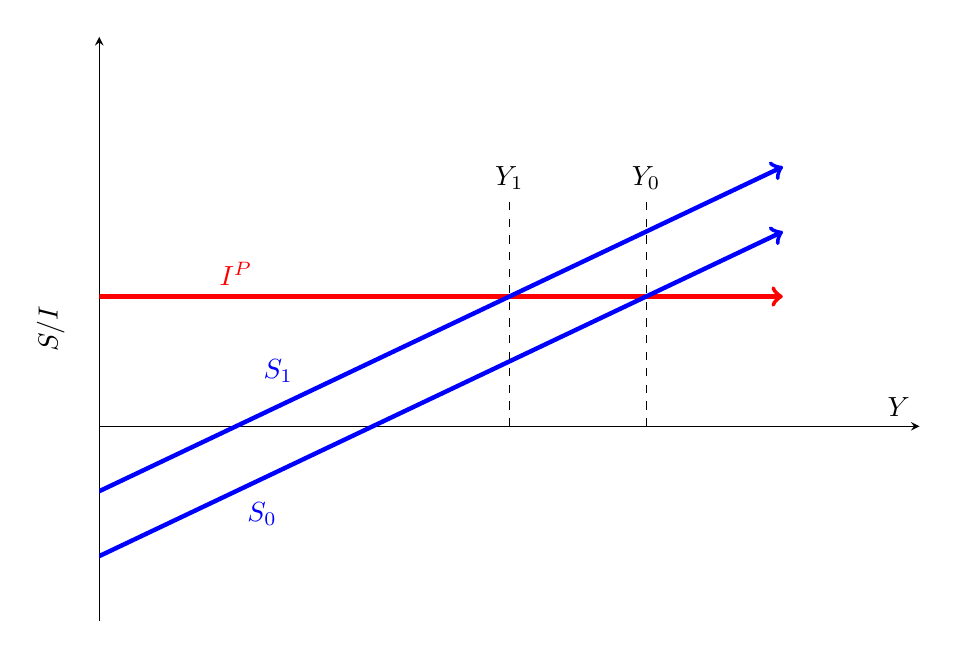
\begin{tikzpicture}
        \begin{axis}[
            xmin = 0,
            xmax = 6,
            ymin = -3,
            ymax = 6,
            width = 12 cm,
            height = 9 cm,
            xlabel = \(Y\),
            xlabel near ticks,
            xtick style = {draw = none},
            xticklabels = \empty,
            axis x line = middle,
            ylabel = \(S / I\),
            ylabel near ticks,
            ytick style = {draw = none},
            yticklabels = \empty,
            axis y line = left,
            samples = 500
        ]

            \addplot[ultra thick, red, ->] coordinates {(0, 2)(5, 2)}
            node[above, pos = 0.2] {\(I^P\)};
            \addplot[ultra thick, blue, ->] {x-2} 
            node[below right, pos = 0.6] {\(S_0\)};
            \addplot[ultra thick, blue, ->] {x-1}
            node[above left, pos = 0.65] {\(S_1\)};
            \addplot[black, dashed] coordinates {(3, 0)(3, 3.5)}
            node[above] {\(Y_1\)};
            \addplot[black, dashed] coordinates {(4, 0)(4, 3.5)}
            node[above] {\(Y_0\)};
        \end{axis}
    \end{tikzpicture}
\end{center}

Here, \(S_0\) has a higher \(\bar{C}\) value than \(S_1\), and therefore has a
lower rate of saving. Because we know that \(S = I^P\), we know that the 
intercept of this saving function with the exogenous firm investment must be at
the output level of the economy, and we can therefore see that a higher rate of
saving implies a lower total output. However the amount of saving undertaken at
each point is the same. \par
This is known as the \textit{paradox of thrift}; it is
an observation that when increased saving is desireable, the real world result
is that no real increase to saving occurs and therefore output falls. This is
to some degree likely a result of the simplicity of the model; it doesn't 
consider supply side factors or changing prices.

\subsubsection*{The Multiplier}

Returning once again to our two sector economy, we have the equation
\[Y = \bar{C} + cY + I^P\]
Which implies that \(Y\) can be calculated as
\[Y = \frac{\bar{C} + I^P}{1 - c}\]
\[\dd{Y}{I^P} = \frac{1}{1 - c}\]
This implies that an increase in \(\bar{C}\) or \(I^P\) leads to an increase in
output. More generally it is taken that a change in an exogenous expenditure in
an economy results in an increase in income, results in an increase in 
consumption, results in a significant increase in total output. The fact of
this increase being larger than the initial change in expenditure is known as
the multiplier. This applies both ways; a reduction is exogenous expenditure is
worse than it would suggest at face value. \par
The magnitude of this multiplier is given by the derivative of \(Y\) with
respect to \(I^P\) shown below the equation; because \(0 < c < 1\) this value
is greater than \(1\) and acts as a multiplier for the increased investment.

\begin{econplot}{\(Y\)}{\(Y / PAE\)}
    \addplot[ultra thick, red, ->, name path = y] {x}
    node[below right, pos = 0.6] {\(Y\)};
    \addplot[ultra thick, blue, ->, name path = lo] {0.5*x+1}
    node[below right, pos = 0.8] {\(\bar{C} + cY + I^P_0\)};
    \addplot[ultra thick, blue, ->, name path = hi] {0.5*x+2}
    node[above left, pos = 0.7] {\(\bar{C} + cY + I^P_1\)};
    \addplot[black, dashed, name path = steps] coordinates 
    {(2, 2)(2, 3)(3, 3)(3, 3.5)(3.5, 3.5)(3.5, 3.75)(3.75, 3.75)(3.75, 3.875)
    (3.875, 3.875)};

    \path[name path = step1] (axis cs: 2, 3) -- (axis cs: 3, 3);

    \node[left] at (axis cs: 2, 2.5) {\(\Delta I^P\)};

    \addplot[fill = red, opacity = 0.3] fill between [
        of = step1 and y,
        soft clip = {domain = 2:3}
    ];
    \addplot[fill = red, opacity = 0.1] fill between [
        of = hi and step1,
        soft clip = {domain = 2:3}
    ];
    \addplot[fill = red, opacity = 0.1] fill between [
        of = hi and y,
        soft clip = {domain = 3:4}
    ];
\end{econplot}

This plot showcases the multiplier effect in response to a change in planned
investment \(\Delta I^P\) from \(I^P_0\) to \(I^P_1\). The dark red shaded 
area is the initial effect of the increased investment, while the light red 
shaded area is the multiplier benefit from the increase. Each ``step'' 
represents the effect of a calculation cycle of increased income implying 
increased consumption implying increased output. \par
This model can be extended to include all of the components of an economy, 
yielding the equation that
\[Y  = \frac{\bar{C} + I^P + G + X - cT}{1  - c(1 - t)}\]
\[\dd{Y}{I^P} = \frac{1}{1 - c(1 - t)}\]
It should be noted that this applies equivalently to all terms in the 
numerator; not just \(I^P\) but also \(\bar{C}\), \(G\), etc. Thus, the 
multiplier is affected by the marginal taxation rate. The taxed income doesn't
go towards an increase in output. The taxation rate can be thought of as a 
dampener on the multiplier. \par
An increase in \(c\) implies an increase in the multiplier, while an increase
in \(t\) implies a fall in the multiplier.

\subsection*{Fiscal Policy}

Fiscal policy can be simplified down to the size of aggregate government
spending, in addition to the quantity of tax and transfer payments made. In
this subject, we generally look at the impact of these different quantities on
the output of an economy. \par
Fiscal policy as a concept is often dated back to Keynes contributions, as
he argued that market failures were the cause of many economic fluctuations,
and that government spending could be modified to address then. Since then a
shift toward monetary policy has occured, though the GFC started the pendulum
back somewhat toward the other direction. \par
In simple terms, in an ideal world output is equivalent to potential output. In
the case that output is below this value, an increase in government spending
can increase planned aggregate expenditure and therefore total output per 
\(Y = PAE\). \par
Some economists argue that this is oversimplified; it has unnacounted for
impacts on the supply side of a market, and it ignores the time lag involved
with government spending.

\subsubsection*{Austerity}

After the Global Financial Crisis, Australia had a somewhat different response
to some other parts of the world. Where Australia increased welfare payments
and government spending to attempt to mitigate a recession, the United Kingdom
adopted a contractionary footing and attempted to reduce government spending
and transfers. \par
As a result of this policy, Australia suffered only a single quarter of
negative growths while the United Kingdom entered a significant recession.
Various perspectives on the correct response to economic downturn do however
exist. This is in part because it is very difficult to isolate variables in
these systems. It is also very difficult to experiment in macroeconomics;
systems on the scale of nations are somewhat difficult to obtain. \par
The general concept of Keynesian fiscal policy is that rather than maintaining
a roughly constant rate of government spending, throughout peaks and troughs
of the business cycle, a government should spend less during booms and spend
less during busts. \par
A concept in fiscal policy is that of \textit{automatic stabilisers}. An
example of this is taxation policy, particularly progressive taxation policy.
These are schemes which will ``automatically'' modulate government spending
according to the state of the economy; for the taxation example, people earning
more pay more tax, essentially reducing government spending.

\subsubsection*{Debt and Fiscal Policy}

Debt is import to fiscal policy as it is one of the two ways money can be 
raised for government spending. Governments can either raise tax rates or sell
bonds to borrow money. Often raising taxation has the issue of disincentivising
labour, an often undesireable outcome. To quantify debt, we use this model
for the debt taken on by a government in time period \(t\)
\[B_t - B_{t - 1} = G_t + Q_t rB_{t - 1} - T_t\] 
Here, \(B_t\) is the government debt at the end of the period, \(G_t\) is total
government expenditure (again, in the period), \(Q_t\) is transfer payments
like welfare, \(r\) is the real rate of interest, \(B_{t - 1}\) is the total
government debt in the previous period and \(T_t\) is total government revenue
(generally taxation) in the period.

\subsubsection*{COVID Response}

The Australian governments response to COVID has largely come in the form of
JobKeeper and JobSeeker, which serve to maintain business relationships and
therefore maintain employment, in addition to offer unemployment insurance;
effectively a safety net for the unemployed. This policy should allow the 
economy to recover more rapidly after the pandemic. \par
While large quantities of debt have been taken on by the government, the 
real interest rate is currently fairly low. In addition, Australia had a
relatively low debt rate prior to the pandemic, and so doesn't suffer overmuch
by comparison when taking on additional debt.

\subsection*{Financial Markets and Intermediation}

When an individual saves money, that money must go somewhere while it is
stored. This money is usually loaned out to people looking to go into debt.
For a saver, it is ideal that the interest rate they earn on these funds is
as high as possible, while for the person taking out a loan to invest this
interest rate would ideally be a minimum. \par
This is a somewhat different relationship to a normal purchase; it suffers from
information asymmetry, where a saver has little information as to the trust-
worthiness of someone they are loaning to. In addition, a significant portion
of debt demand is in the form of extremely large sums for very large projects,
while much of saving is done by small (household) groups. Financial
intermediation exists to facilitate this.

\subsubsection*{Financial Intermediaries}

Financial intermediaries are primarily banks, but can also include credit
unions. Banks accept deposits from savers, paying them a low interest rate
on their savings while lending them out at a higher interest rate to investors.
The spread between these two interest rates is the bank's cut and is the source
of its profits. Generally the more transactions a bank undertakes the more
profitiable it is, but this does come with some risk. \par
The specialisation of the bank is in evaluating risk, and in pooling savings of
small individual savers. This can minimise the risk of a single project, as
well as funding large projects and making risk management more efficient.

\subsubsection*{Financial Markets}

Another financial intermediary is in financial markets. These include
\begin{itemize}
    \item Bond markets where large business sell bonds at a given price with 
        a commitment to pay back a larger some at some fixed future date.
    \item Stock markets where firms offer a share of firm profit in exchange
        for an upfront sum. These are generally more risky than bonds, but
        offer a higher rate of return.
\end{itemize}
When working in these markets, legislation requires that businesses must
provide a \textit{prospectus} which provides information about a business.
These markets play an important role in allowing savers to diversify their
saving portfolios. \par
Conceptually, these markets will tend to finance the most profitable projects
as these are the ones that will tend to be invested into. This has the added
benefit of maximising rate of return for savers. \par
This system can be severely damaged during market crashes like that 1929
market crash in the US, or during the GFC. Here, issues with banks and other
intermediaries can cause failures in this transfer of wealth, leading to a
contraction in investment and consumption and thus overall market contraction.

\subsection*{Money}

Money fulfills a few important roles in society
\begin{itemize}
    \item It stores and transfers purchasing power over time. It should
        therefore be long lasting and durable.
    \item It is also a unit of account; a measure of the economic value of a
        good.
    \item It is a medium of exchange, it allows people to exchange a common
        good for other goods, avoiding the inefficiences of a barter economy.
\end{itemize}
Thus money includes currency, but also bank deposits, the two of which are
combined to make \(M1\), or for \(M3\) including private non-bank deposits.
\textit{Broad money} describes \(M3\) as well as borrowings from the private
sector, minus holdings of currency and deposits of non-bank depository
corporations. \par
Banks have a special role in a macroeconomy in that they create money. They
do this under a system of \textit{fractional reserve banking}. Under this
system, banks take deposits from the public, keeping a certain percentage of
these deposits on hand, but lending out the majority. These loan funds end up
being re-deposited elsewhere and the process repeats. This essentially results
in a multiplier to the quantity of money in circulation. \par
This means that if every customer wants to withdraw their savings
simultaneously, the bank would be unable to make good on the deposits. The
ability of the banks to create money is controlled by the amount they are
required to keep on reserve. A bank will generally want to have as many loans
as possible.

\subsubsection*{Quantity Theory of Money}

The quantity theory of money states
\[MV = Py\]
Here, \(M\) is the money supply, \(V\) is \textit{velocity}, a measure of the
amount of transactions that can be financed from a given amount of money in
some time period. \(P\) is the price level and \(y\) is the real output of the
economy. \(V\) is affected by the structural features of an economy, such as
the ease of the payment mechanisms. If \(V\) and \(y\) are fixed in the short
run, there is a direct relation between \(M\) and \(P\). \par
This is often a desireable outcome, however it can be difficult to control
velocity.

\subsubsection*{The Reserve Bank}

The Reserve Bank of Australia is the central bank, an institution which
controls monetary policy for the nation. It has severy important functions
\begin{itemize}
    \item It controls the level of the nominal interest rate
    \item Historically it has controlled the level of money supply
    \item Some central banks directly control the exchange rate
    \item It also regulates payment systems and financial stability
\end{itemize}
The goals of a central bank are generally to maintain stability of the currency
(i.e. low inflation), to try and keep employment levels high (i.e. close to the
natural rate of unemployment). \par
The way the central bank manages the interest rate is by trying to target the
interest rate in overnight unsecured interbank market. Transactions in this
space occur through the Exchange Settlement Accounts of banks, which are used
to settle balances incurred between banks by customers of these banks each
evening. The accounts must remain positive, but holding large somes in them is
prohibitive due to the foregone interest this entails. Because the central bank
controls money supply in this arena, it has control over this interest rate.
\par
This interest rate tends to control the other interest rates in the economy.
The interest rate for this market is known as the cash rate, and it has a very
significant impact on other loan types. This is largely due to arbritrage, the
process of market factors altering prices through competition. \par
Today, the central banks main goal is \textit{inflation targeting} where the
bank tries to set an inflation rate over the business cycle. It is felt that
this is a better metric than money supply because it is more explicit and thus
offers better evaluation. It is also thought to be good for stability; with a
set target people can have well defined expectations for the inflation of their
money. \par
Over the course of this subject, we assume that the central bank can control
real interest rates. In reality, the market for loanable funds means this isn't
quite too; while the central bank can more or less set the nominal interest
rate, they have less control over the real interest rate.

\subsubsection*{Consumption and Interest Rates}

\[C^d = \bar{C} + c(Y - T)\]
This is the basic model for Keynesian consumption, while the more complex
version, accounting for saving, takes the form
\[C^d = \bar{C} + c(Y - T) - \gamma_cr\]
Where \(\gamma_c\) is, a coefficient relating consumption to the
real interest rate, \(r\). Also in this situation, we consider that investment
of firms has an opportunity cost of lost interest. Thus
\[I^P = \bar{I} - \gamma_Ir\]
Thus firms have some maximum investment \(\bar{I}\), reduced by the amount
saved according to \(\gamma_Ir\). A low interest rate would therefore encourage
increased consumption. However often \(\gamma_I\) and \(\gamma_c\) are very
small. \par
In a three sector economy, our model now looks like
\[PAE = C^d + I^P + G =\bar{C} + c(Y - T) -\gamma_cr + \bar{I} -\gamma_Ir + G\] 
In this model, an increase in \(r\) implies a drop in \(PAE\), the magnitude of
which is dependent on the \(\gamma\) terms.

\subsubsection*{Behaviour of the Reserve Bank}

The behaviour of the reserve bank can be quantified through the equation
\[r_t = \bar{r} + \alpha_y\left(\frac{Y - Y^*}{Y^*}\right) + \alpha_\pi\pi\]
Here, \(r_t\) is the real interest rate targeted by the reserve bank,
\(\bar{r}\) is a constant, \(\alpha_y\) is a constant greater than \(0\) which
relates interest rates to the output gap (i.e. the fractional \(Y\) term),
\(\alpha_\pi\) is another constant greater than \(0\) which defines how
interest rates respond to inflation. \par
The RBA wants to try and keep output near potential, to ensure stability of
unemployment. If \(Y > Y^*\), an increase in \(r\) occurs due to the positive
\(\alpha_y\) term, tending to reduce \(PAE\), while if output is below
potential, the term is negative resulting in a drop in \(r\), and an increase
in \(PAE\). \par
For the \(\alpha_\pi\pi\) term, if \(\pi\) is high, and increase in \(r\)
occurs, resulting in a fall in output and a reduction in inflation pressures.
When \(\pi\) drops, so too does \(r\) resulting in an increase in demand and
thus inflation. This will tend to react aggressively; generally a change in
\(\pi\) is reflected by a larger change in \(r\). \par
This description is approximate; the reserve bank still has plent of leeway
for human intuition. Interestingly, \(0\) is not a lower bound for the interest
rate. Economists tend to think that a slightly negative interest rate is
acceptable due to the utility inherent in storage of wealth in a bank.

\subsection*{Aggregate Demand and Supply}

The Keynesian model makes the assumption that prices in an economy are fixed in
the short run. The model of aggregate supply and demand allows us to consider
situations with high inflation or other price changing factors. Aggregate
demand and supply is essential to understanding evens like the GFC.

\subsubsection*{Aggregate Demand}

The model of aggregate demand assumes that
\begin{itemize}
    \item Household consumption is given by 
        \(C^d = \bar{C} + c(Y - T) - \gamma_cr\)
    \item Firm investment is given by \(I^P = \bar{I} - \gamma_Ir\)
    \item Government, export and import spending is exogenous
    \item The monetary policy of the system is defined by the policy reaction
        function.
    \item Prices are set by the aggregate of firms in the economy.
\end{itemize}
The model has implications for the level of output of the economy, as well as
the level of inflation implied by the model. It therefore has implications for
the real interest rate as well as consumption. \par
The aggregate demand curve exists with one axis showing output and another
showing inflation. It maps the set of points where \(PAE = Y\), points in
Keynesian equilibrium; no unwanted change to inventory occurs. \par
The plot will
take the form of a downward curve. A high level of inflation implies a low
level of output, a fact largely due to the effects of monetary policy from the
reserve bank. The reserve bank will respond to high inflation by attempting to
lower output, resulting in a lower level of output at higher levels of
inflation. \par
On an individual level, it is intuitive that inflation coincides with erosion
of wealth, reducing people's ability to consume. In addition, generally those
that are wealthy are able to make intelligent investment decisions that protect
them from inflation, while the poor are less able to do this. This, combined
with the fact that the consumption of wealthier people tends to be less tied
to increases in their wealth explains a fall in output.

\subsubsection*{Shocks to the Aggregate Demand Curve}

Causes of shifts to the aggregate demand curve include
\begin{itemize}
    \item Shifts to the planned aggregate expenditure curve, excluding those
        caused by inflation. These include changes in household behaviour, firm
        behaviour or exogenouse variables. Changes inflation cause a move along
        the same curve.
    \item Exogenouse changes to the policy reaction function of the central
        bank. If the relationship between the real interest rate and inflation
        changes, so too will the aggregate demand curve.
\end{itemize}

We can examine the effect of a change in exogenous expenditure through a case
study.

\begin{econplot}{\(Y\)}{\(Y/PAE\)}
    \addplot[red, ultra thick, ->] {x}
    node[above left, pos = 0.95] {\(Y\)};
    \addplot[blue, ultra thick, ->] {0.4*x + 2}
    node[above left, pos = 0.7] {\(PAE(G_1, \pi)\)};
    \addplot[blue, ultra thick, ->] {0.4*x + 1}
    node[below right, pos = 0.85] {\(PAE(G_0, \pi)\)};
    \node[circle, fill, inner sep = 2pt] at (axis cs: 1.67, 1.67) {};
    \node[below right] at (axis cs: 1.67, 1.67) {\(Y_0\)};
    \node[circle, fill, inner sep = 2pt] at (axis cs: 3.33, 3.33) {};
    \node[above left] at (axis cs: 3.33, 3.33) {\(Y_1\)};
\end{econplot}

Here, government expenditure has increased from a level \(G_0\) to a level
\(G_1\), causing an increase of output from level \(Y_0\) to \(Y_1\). This all
occurs at a constant inflation rate \(\pi\). The below plot shows the impact of
this change in \(PAE\) in the aggregate demand curve.

\begin{econplot}{\(Y\)}{\(\pi\)}
    \addplot[blue, ultra thick, domain = 1.25:5, <->] {0.1*(x - 9)^2};
    \addplot[blue, ultra thick, domain = 1:5, <->] {0.1*(x - 8)^2};
    \addplot[black, ultra thick, dashed] coordinates {(0, 2.5)(5, 2.5)};
    \node[circle, fill, inner sep = 2pt] at (axis cs: 3, 2.5) {};
    \node[below left] at (axis cs: 3, 2.5) {\((Y_0, \pi)\)};
    \node[circle, fill, inner sep = 2pt] at (axis cs: 4, 2.5) {};
    \node[above right] at (axis cs: 4, 2.5) {\((Y_1, \pi)\)};
    \addplot[black, thick, ->] coordinates {(2.2, 3.5)(2.9, 3.5)};
\end{econplot}

We can see that because the inflation rate \(\pi\) has remained constant while
the level of output increases, the curve has moved to the right, to a higher
level of output. Generally a rise in \(PAE\) implies a shift outward of
aggregate demand while a fall in \(PAE\) implies a shift inward. \par
Another way the curve can be affected is through changes in the policy reaction
function of the central bank. This can be considered by thinking about what the
new function entails for saving and expenditure behaviours. For example a
decrease in real interest rate implies an increase in \(PAE\) implying a
rightward shift of the demand curve.

\subsubsection*{Aggregate Supply}

The aggregate supply curve maps out a set of points \((Y, \pi)\) where firms
production decisions are consistent with price changes. The prices set by firms
are determined by costs of production, particularly labour costs. They are also
influenced by demand for their products. \par
In general, inflation will tend to behave as though it has inertia; it will
be slow to change naturally. \par
The primary determinant of production costs is the cost of labour.
\[Y = wL + rK\]
Tells us that total output is made up of wages paid for labour and interest
paid on capital, with \(55-60\%\) of this made up by the labour term. These
wages are generally negotiated between businesses and workers, and tend to
be inflexible in the short term. \par
The \textit{real wage} describes the distribution of gains from trade between
workers and employers. If we assume that the two can agree on a fair real wage
(which assumes that workers will have some insight into the future, considering
inflation, etc for calculation of nominal wage.). This implies that high
inflation needs high nominal wage increases to compensate, while low inflation
implies low nominal wage increases. \par
This forms a kind of self-fulfilling
prophecy; an expectation of high prices results in higher wages and higher
costs of production implying high prices. Thus the expectation of inflation in
some way dictates the rate of inflation. \par
But what determines this expectation? Considering inflation inertia, one would
expect the present rate of inflation to reflect future inflation. Thus if
inflation inertia is the main factor, we can calculate inflation through
\[\pi^e_t = \pi_{t - 1}\]
\[\pi_t = \pi^e_t + \epsilon_t\]
\[\pi_t = \pi_{t - 1} + \epsilon_t\]
Here, \(\pi^e_t\) is the expected rate of inflation during time period \(t\),
set equal to the rate of inflation in period \(t - 1\). We then set \(\pi_t\)
equal to this value plus some exogenous constant \(\epsilon_t\), which
represents external shocks to the system. \par
\(\epsilon_t\) could be made up of oil price shocks, natural disasters or
surprising wage bargaining outcomes. \par
In addition to labour considerations, the desired output level of firms is
dependent on product market conditions. If firms have lower demand they will
tend to lower prices to try and drive demand and thus lower inflation. Thus
when output is equal to potential or desired output inflation will be
unaffected by the product market. However if output is above potential, firms
will raise prices resulting in increased inflation. Inversely, lower output 
will result in lower prices and lower inflation. \par
Considering this, we can develop an equation for the inflation rate with
respect to expectations and the product market.
\[\pi_t = \pi_{t - 1} + \gamma\left(\frac{Y_t - Y^*}{Y^*}\right) + \epsilon_t\]
Where \(\gamma\) describes the responsiveness of inflation to deviations in the
output gap.

\begin{econplot}{\(Y\)}{\(\pi\)}
    \addplot[red, ultra thick, ->] {x}
    node[below right, pos = 0.9] {\(\pi(\gamma_0)\)};
    \addplot[red, ultra thick, ->, domain = 0:4] {3*x/2 - 1}
    node[above left, pos = 0.8] {\(\pi(\gamma_1)\)};
    \addplot[black, ultra thick, dashed] coordinates {(0, 2)(4, 2)}
    node[right] {\(\pi_{t - 1} = \pi^e_t\)};
    \addplot[black, ultra thick, dashed] coordinates {(2, 0)(2, 3)}
    node[above] {\(Y^*\)};
\end{econplot}

Here \(\gamma_0 < \gamma_1\), so the \(\gamma_0\) curve is less responsive to
changes in \(Y\) and thus has a lower gradient. The two intersect at \(Y^*\).
The gradient of each curve is not exactly \(\gamma\) but rather some function
of \(\gamma\). At the output level \(Y^*\) the output dependent term is \(0\)
so \(\gamma\) has no effect. At this level, it is exclusively \(\pi^e_t\) and
\(\epsilon_t\) which determine the inflation level. Because \(\epsilon_t\) is
taken to be \(0\) for the above plot, the two are simply equal.

\subsubsection*{Shocks to the Aggregate Supply Curve}

Shocks to this curve might happen for a variety of reasons. These include
supply side changes, like new resources or improved technology or changes to
regulation. For example immigrant labour might increase potential output or 
Covid-19 lockdown regulations migth reduce potential output. Changes to
inflation expectations in addition to exogenous inflation shocks have
significant effects. \par
When potential output increases, the supply curve is directly shifted to the
right; this can be easily understood by understanding that the potential output
\(Y^*\) pegs the curve, and so moving it shifts the curve. \par
If expected inflation \(\pi^e_t\) increases, the curve will shift upward or
equivalently left. It will move up by exactly \(\Delta\pi^e\), again because
the point \((\pi^e_t, Y^*)\) always lies on the curve. \par
An inflation shock to \(\epsilon_t\) will have the same behaviour.

\subsection*{Equilibrium of Aggregate Supply and Demand Curves}

The goal of a theory of business cycles is to be able to describe the causes of
output fluctuations. This can be explained through shifts in the aggregate
demand and supply curves. \par
For the two curves to be in equilibrium, output must equal planned aggregate
expenditure and firms pricing structures must be consistent with their desires.
For a long run equilibrium, these must be satisfied however additionally there
must also be a consistent trend of expected levels of inflation
(\(\pi = \pi^e\)), Adjustment from a short run equilibrium to a long run
equilibrium is undertaken by moderation of inflation. \par
We can consider as an example a drop in consumer spending.
\[C^d = \bar{C} + c(Y - T) - \gamma_cr\]
i.e. a reduction in \(\bar{C}\). This will have the effect of a reduction in
aggregate demand. This will imply a build up of inventories for firms,
resulting in a drop in rate of increase of prices (i.e. inflation). This
decline will be mitigated by the policy reaction function, causing the real
interest rate to drop and thus investment to increase.

\begin{econplot}{\(Y\)}{\(\pi\)}
    \addplot[blue, ultra thick, domain = 1.25:5, <->] {0.1*(x - 9)^2 - 1}
    node[above right, pos = 0.9] {\(AD(\bar{C}_0)\)};
    \addplot[blue, ultra thick, domain = 1:4.5, <->] {0.1*(x - 8)^2 - 1}
    node[below left, pos = 0.8] {\(AD(\bar{C}_1)\)};
    \addplot[red, ultra thick, ->, domain = 0:4.5] {x + 1}
    node[above left, pos = 0.8] {\(AS\)};
    \node[circle, fill, inner sep = 2pt] at (axis cs: 2.38, 3.38) {};
    \node[right, xshift = 0.2cm] at (axis cs: 2.38, 3.38) {\((Y^*, \pi_0)\)};
    \node[circle, fill, inner sep = 2pt] at (axis cs: 1.82, 2.82) {};
    \node[left, xshift = -0.2cm] at (axis cs: 1.82, 2.82) {\((Y_1, \pi_1)\)};
    \addplot[black, thick, <-] coordinates {(1.25, 3.75)(2, 3.75)};
    \addplot[black, thick, <-] coordinates {(2.7, 2)(3.4, 2)};
\end{econplot}

The above plot depicts the changes as the curve shifts from output level
\(Y^*\) to \(Y_1\). The end result is a fall in aggregate demand cause a fall
in output and inflation level. This is a short-run result; because
\(\pi_1 < \pi^e\) this cannot be a long term equilibrium. \par
In general, we expect inflation and inflationary expectations to return the
economy to long run equilibrium. In the case that \(Y < Y^*\) as above, the
economy will tend to have a falling inflation and inflationary expectations
and thus the economy will return to a long-term equilibrium. When \(Y > Y^*\)
inflationary expectations will tend to increase, and the economy will once
again self correct. \par
So essentially what happens is that the supply curve responds to a change in
inflationary expectations by falling, which eventually leads to a new long term
equilibrium when \(AS = AD = \pi^e\). \par
In general, the key adjustment in the system is the change of expected
inflation over time resulting in a return to long term equilibrium.

\subsubsection*{Implications}

Changes in aggregate demand will generally cause output and inflation to move
in the same direction. Changes in aggregate supply will tend to cause output
and inflation to move in opposite directions. The overall impact of an shock to
supply or demand is dependent largely on the size of the shock, as well as the
relative slopes of aggregate supply and demand. \par
This makes sense; a steeper sloped curve will result in a larger shock
comparative to a flatter curve, all else equal. \par
Keynesian policy is relevant to this process because generally the adaptation
back to a long term equilibrium is quite slow, due to long term contracts and
other factors. In this situation, we may have \(u > u^*\), which is unpleasant.
Through Keynesian policy, we can try to reduce \(u\) or moderate \(Y\) while
the economy returns to equilibrium. \par
If however we accept that rapid price adjustment is the major factor in
equilibrium, government intervention is less important and can indeed be seen
to be undesireable. Which of these two takes is correct is an important issue
in macroeconomics. Most economists tend to agree that intervention is
productive however.

\subsubsection*{Phillips Curve}

The Phillips curve shows a relationship between a low level of unemployment and
a high level of inflation. This relationship has grown weaker over time.

\section*{Economic Growth}

Economic growth has not been a constant over time. Until around 1750 C.E.,
there was little economic growth. With the advent of the industrial revolution
in primarily western Europe, sustained growth occured in countries like Britain
and Germany. As the growth spread to some other countries and accelerated, a
large divergence in wealth occured between 1800 and 1950. \par
Output per capita is an important determinant of many important factors,
including health and nutrition or education. Over time, countries are tending
to become more similar in terms of per capita output. \par
Even small differences in economic growth can lead to quite different outcomes.
For example, where Japans per-capita ouput was only a quarter of Australia's
around 1900, it has rapidly increased in the post-WW2 period to around the same
figure. \par
Where the study of business cycles focussed on deviations from potential
output and on the possibility of market failures, with fixed prices, with the
goal of identifying effective govenrment intervention, the study of economic
growth addresses changes in potential output with time and assumes adjustment
of prices will mitigate market failures.

\subsection*{Productivity}

We can represent output per capita as
\[\frac{Y}{P} = \frac{Y}{N}\cdot\frac{N}{P}\]
Here, \(N\) is the number of employed workers. \(\frac{Y}{N}\) is labour
\textit{productivity}, units of output per worker. \(\frac{N}{P}\) is the
employment to population ratio. We can thus see that product per capita will
be affected by worker productivity changes or employment ratio changes. \par
Productivity might be increased by something like improved technology, while
employment to population is somewhat more difficult to increase. Interestingly
labour productivity growth has slowed down somewhat since the GFC; some argue
that this is due to mismeasurement due of digital products. Others argue that
the reduction is still due to the GFC, while still others argue that new
technology is becoming more difficult to discover and we will suffer a long
term reduction in labour productivity growth. \par
This may be due to factors like further required education to reach the
forefront of a field with advancing science and technology. \par
Other factors of productivity include institutions like political and legal
environment, human capital (skills, training of workers), physical capital,
land and natural resources, etc.

\subsubsection*{Production Function}

Much of economic growth uses an \textit{aggregate production function}
\[Y_t = A_tf(K_t, L_t)\]
Where \(Y_t\) is output in time period \(t\), \(A_t\) is a measure of
productivity (technology, etc), \(K_t\) is capital stock and \(L_t\) is labour
force (factors of production). \(f\) is a production function which states
how much \(K_t\) and \(L_t\) are able to produce. The Cobb-Douglas production
function for instance looks like
\[Y_t = A_tK_t^\alpha L_t^{(1 - \alpha)}\]
Where \(\alpha\) is a constant defining how relatively important labour and
capital are. \(0 < \alpha < 1\). The function generally assumes the marginal
products of labour and capital are positive, and that they are decreasing.
Equivalently this states that their first derivatives are positive and second
derivatives are negative. \par
Another assumption is that the function has a constant return to scale, i.e.
\[f(K, L) = Y \Rightarrow f(xK, xL) = xY\]
This has some useful implications
\[\frac{Y_t}{L_t} = \frac{f(K_t, L_t)}{L_t} 
= f\left(\frac{K_t}{L_t}, 1\right)\]
This tells use that output per worker depends on capital per worker but not on
the size of the economy. In the Cobb-Douglas function we find that
\[Y_t = A_tK_t^\alpha L_t^{(1 - \alpha)} \Rightarrow \frac{Y_t}{L_t} 
= A_tK_t^\alpha L_t^{-a} = A_t\left(\frac{K_t}{L_t}\right)^\alpha\]
Once again, it is evident that the size of output per capita is dependent on
capital to worker ratio. If we plot output per worker against capital per
worker, the curve will have an increase value with a decreasing slope.

\subsubsection*{Solow-Swan Model}

The Solow-Swan model examines the relationship between variables like output
per capita, savings rate, population growth and productivity. It highlights
the importance of productivity growth for living standards. \par
The model begins with an initial capital stock \(K_0\) and a level of labour
\(L_0\) and attempts to describe how these values change over time. To explain
this it makes assumptions with respect to the production function and behaviour
of households within the economy. \par
The model uses the aggregate production function approach of
\[Y_t = Af(K_tL_t)\]
Where \(A\) is \textit{total factor productivity} a coefficient describing the
overall productivity due to factors like technology and regulations. This
displays the behaviour previously highlighted; positive first derivative and
negative second derivative, in a addition to constant returns to scale. \par
The model describes a capital accumulation function of
\[K_{t + 1} = (1 - d)K_t + I_t\]
Where \(d\) is the depreciation rate and \(I_t\) is the amount invested in
period \(t\). Finally, the model uses a labour growth model with a function
\[L_{t + 1} = (1 + n)L_t\]
Where \(n\) is the growth rate of labour. The model assumes a constant saving
rate given by \(\theta\), the marginal propensity for saving. This means that
\(c\), the marginal propensity for consumption is given by \(1 - \theta\). It
additionally assumes full employment of capital and labour. It finally assumes
that saving is equal to investment, that is
\[\theta Y_t = I_t\]
If we take our equation for capital growth and divide through by labour force,
we can find the growth in capital per labour.
\[K_{t + 1} = (1 - d)K_t + I_t\]
\[\frac{K_{t + 1}}{L_{t + 1}} = \frac{(1 - d)K_t + I_t}{L_{t + 1}} 
= \frac{(1 - d)K_t + \theta Y_t}{(1 + n)L_t}
= \frac{1 - d}{1 + n}\frac{K_t}{L_t} + \frac{\theta}{1 + n}\frac{Y_t}{L_t}\]
\[\Rightarrow \Delta\frac{K_t}{L_t} = \frac{K_t + 1}{L_t + 1} - \frac{K_t}{L_t}
= \left(\frac{1 - d}{1 + n} - 1\right) \frac{K_t}{L_t}
+ \frac{\theta}{1 + n}\frac{Y_t}{L_t}\]
If we observe that \(n\) is generally quite small, being the population growth
rate, then \(1 + n \approx n\) means that we can rewrite the above as
\[\Delta \frac{K_t}{L_t} = \theta\frac{Y_t}{L_t} - (d + n)\frac{K_t}{L_t}\]
Where the left term on the right side is savings per worker, and the right term
is \textit{replacement investment}. This replacement investment is the amount
of investment required to keep the capital to labour ratio a constant. The
Solow-Swan model looks for a situation where this change in the capital to
labour ratio is \(0\).

\begin{econplot}{\(\frac{K}{L}\)}{\(\frac{Y}{L}\)}
    \addplot[red, ultra thick, ->, domain = {0:3.9}] {3*x^0.5}
    node[below right, pos = 0.95]
    {\(\frac{Y}{L} = Af\left(\frac{K}{L}, 1\right)\)};
    \addplot[blue, ultra thick, ->] {x^0.5}
    node[below, pos = 0.95] {\(\theta\frac{Y}{L}\)};
    \addplot[red, ultra thick, ->] {0.75*x}
    node[below right, pos = 0.95] {\((n + d)\frac{K}{L}\)};
    \addplot[black, ultra thick, dashed]
    coordinates {(1.78, 0)(1.78, 4)(0, 4)};
    \node[circle, fill, inner sep = 2pt] at (axis cs: 1.78, 4) {};
    \node[above left] at (axis cs: 1.78, 4)
    {\(\left(\frac{Y}{L}\right)^*, \left(\frac{K}{L}\right)^*\)};
    \node[circle, fill, inner sep = 2pt] at (axis cs: 1.78, 1.33) {};
\end{econplot}

By plotting replacement investment, saving per working and output per worker
we can find the equilibrium outcome of this system. At the intersection of
saving per worker and replacement investment we find the equilibrium level
of capital per worker. A the same capital per worker value, we find the
equilibrium level of output per worker. The output per worker level of the
equilibrium point is the level of savings per worker, while the distance
between the two marked points is the level of consumption per worker. \par
In the case that savings per worker is more than replacement investment (i.e.
a point on the savings curve left of the equilibrium), quantity of capital will
increase, resulting in a shift into equilibrium. In the case that it is less
than replacement (i.e. to the right of equilibrium), level of capital per
worker will decrease to equilibrium. \par
We can use this plot to perform comparative statics; for instance we can see
that an increase in the saving rate \(\theta\) will effect a shift up in the
saving curve resulting in a higher level of capital to labour and a higher
level of output per worker.

\subsubsection*{Implications}

We have seen that the Solow-Swan model implies a steady-state level of capital
per worker, which the economy will tend to return to. It also implies that
output per worker depends upon capital per worker. \par
We can use the model iteratively to determine values for capital per worker,
output per worker and consumption per worker to describe the economy at each
point of time. \par
The implication of the steady state of the system implies that for output
per worker to change, some exogenous factor like \(\theta\), \(A\) etc must
change. Holding these other variables equal, this implies that the rate of
growth of output is dependent simply on rate of growth of labour
(\(Y^\prime = n\)). \par
The model can be extended by including growth in productivity and output per
worker, which explains how countries can grow richer. The current model only
shows us that capital per labour is less a driver of increased welfare than is
productivity growth.

\subsection*{Empirics of Economic Growth}

The Solow-Swan model suggested that an economy tends toward a steady-state
capital to labour ratio, and indicated that long run growth occurs due to
growth in productivity.

\subsubsection*{Convergence}

Convergence is the idea that countries might become more similar over time.
Absolute convergence suggests that all economies should converge to be more
like each other; in some way, this is a test of the Solow-Swan model; countries
with similar characteristics should tend to similarity. \par
It suggests an inverse relationship between output per worker and growth rate
in similar countries. Statistics from the real world do not support this
outcome; either because the model does not reflect the world very well, or
because countries are not in reality similar in the real world. \par
This leads to the conditional convergence hypothesis; that all economies should
converge to some value, while similar countries should converge to roughly
the same value. When restricting the hypothesis in this way, such as by looking
at ``open economies'', there is more support for it.

\subsubsection*{Growth Accounting}

Growth accounting is a way of splitting output growth into productivity,
capital stock, and labour growth. It is useful because it allows us to gain
insight into what is driving output growth in an economy. It doesn't necessary
account for what is driving these factors; e.g. if an institution has effected
some regulation resulting in improved productivity or some technology has done
so. \par
We begin this analysis with the production function
\[Y_t = A_tf(K_t, L_t)\]
We then take the logarithm of each size, and then differentiate with respect to
time this equation.
\[\log(Y_t) = \log(A_t) + \log(f(K_t, L_t))\]
\[\frac{1}{Y}\dd{Y}{t} = \frac{1}{A}\dd{A}{t} 
+ \frac{1}{f(K, L)}\dd{f(K, L)}{K}\dd{K}{t} 
+ \frac{1}{f(K, L)}\dd{f(K, L)}{L}\dd{L}{t}\]
Here, the terms from left to right are the growth rate of output, the growth
rate of productivity, with the last two terms representing the growth rate of
capital with respect to labour and the growth rate of labour with respect to
capital. In general,
\[\frac{1}{z(t)} \dd{z}{t} = \hat{z}\]
Where \(\hat{z}\) is the growth rate of \(z\) (growth with respect to time).
Using this, and some other manipulations of our original equations we can
rearrange to find the equation
\[\hat{Y} = \hat{A} + \frac{rK}{Af(K, L)}\hat{K} + \frac{wL}{Af(K, L)}\hat{L}\]
To do this, we multiply the two labour and capital terms by \(\frac{A}{A}\) and
use the expressions for the value of \(w\) and \(r\) in a competitive market
given by the marginal products of labour and capital
\[w = A \dd{f}{L}\:\:\:r = A \dd{f}{k}\]
to replace the relevant terms.
\par
We then use the equation \(Y = wL + rK\), divided through by 
\(Y\) (\(= Af(K, L)\)) to
understand \(\frac{wL}{Y}\) as the labour share of output and \(\frac{rK}{Y}\)
as the capital share of output. \par
We can then understand the above equation as stating that the growth rate of
output \(\hat{Y}\) is given by the growth rate of productivity \(\hat{A}\)
multiplied by the capital share, multiplied by growth rate of capita
\(\hat{K}\) multiplied by labour share, multiplied by growth rate of labour,
\(\hat{L}\). \par
Given that we have access to data on output \(Y\) and output growth
\(\hat{Y}\), including labour share and capital share, interest rates \(r\)
and capital stock \(K\), wages \(w\), employment \(L\) and employment growth
\(\hat{L}\), and investment (which implies) \(\hat{K}\), there is only one
unknown \(\hat{A}\), sometimes known as the Solow residual. Thus, this equation
is useful for finding growth in total factor productivity in an economy. \par
Essentially, the equation says all growth in an economy not due to increases
in capital or labour are due to increases in productivity, due to technology,
regulation, etc. \par
One can calculate using margin of error to avoid bias in the estimate of
productivity growth.

\subsubsection*{Applications}

An application of these principles was in the study of the East Asian Tigers;
successful East Asian countries undergoing rapid growth. Much of the success of
these countries could be attributed to increases in capital stock and labour,
with less influence from increases in total factor productivity. The high
saving rates motivated by government policy effected high rates of growth in
capital stock resulting in rapid economic growth. \par
An idea that arises from this result is that increases in savings, while
motivating increases in output per worker in the short term, has long-term
implications that are less favourable.

\section*{International Trade}

Over time, trade has become a more and more important aspect of global
production. The advance of techonologies such as shipping containers or
information technology has also encouraged trade. In addition globalisation
has greatly increased the importance of trade, due to developing economies and
organisations like the World Trade Organisation. \par
In understanding trade, it is important to look at the direction of trade; who
exports what to who, the benefits of trade; i.e. the incentive for countries to
trade, and the effects of trade such as its distributional aspects. \par
In general, trade allows magnification of benefit of production efficiency, in
addition to improving consumption efficiency. There are however distributional
effects; while some gain from trade, others lose out. \par
In an endowment economy, there is a given quantity of each good available. This
is somewhat similar to an economy in autarky; where the country has access only
to the goods which it produces. When an economy engages in trade, is widens the
consumption possibilities from simply these prescribed quantities to those in
addition to whatever they might be traded for.

\subsubsection*{In a Production Economy}

While trade in an endowment economy is relatively simple to understand, in a
production economy we can see the efficiency introduced by trade. In general,
trade allows economies with comparative advantages to produce goods for which
they have this advantage rather than goods it would be less efficient for them
to produce. \par
We do this by calculating the opportunity cost for a given good in terms of
other goods, to find which is the most efficient good for them to produce,
relative to others. In general, everyone will have the comparative advantage in
some arena, even if they have an absolute advantage in none. \par
If we plot production of one good against production of another, we have a
production possibility frontier diagram. We can superimpose these diagrams by
prioritising those with a comparative advantage for production of their
advantaged good to find the maximum consumption for a given pair of goods. This
shows us the benefits of specialisation implicit in trade. \par
Once we add price into our system, we find that if the price of one good is
less than the opportunity cost of that good, production of that good will not
occur. If the price is above the opportunity cost, exclusively production of
that good will occur, with trade used to gain access to other goods (on an
individual level). \par
In a more realistic economy in a large body of workers, the composite
production possibility frontier will display a curved shape with an increasing
gradient (i.e. opportunity cost). Generally, it will be most efficient for an
economy to produce the maximum total value of goods with prices taken as
exogenous, with little regard for what these goods are, as they can then be
traded for other goods. The price information here will perform the allocation
task of determining opportunity cost.

\end{flushleft}
\end{document}
